\chapter{Grundlagen}

Im folgenden Kapitel sollen konzeptionelle Grundlagen erläutert werden, welche für das Verständnis der Bachelorarbeit notwendig sind.
Dabei wird auf die Themen Requirements Engineering, Augmented Reality und die Software reQlab eingegangen.

  \section{Requirements Engineering}
  Die Bachelorarbeit soll sogenannte Requirements, also Anforderungen, visualisieren.
  Daher ist es für das Verständnis der Arbeit wichtig, die Grundlagen des Requirements Engineering zu kennen.

    \titleemph{Requirements}

    Grundlegend sind Requirements Anforderungen, die an ein System gestellt werden.
    Das International Requirements Engineering Board (IREB) definiert sie in ihrem Glossar mit drei Eigenschaften \autocite[][Def. Anforderung]{ireb_cpre_glossary}
    \begin{itemize}
        \item Ein Bedürfnis eines Interesseneigners (Stakeholder).
        \item Eine Eigenschaft oder Fähigkeit, die ein System haben soll.
        \item Eine dokumentierte Repräsentation eines Bedürfnisses, einer Fähigkeit oder einer Eigenschaft.
    \end{itemize}
    

    Sie sollen also die Bedürfnisse der Stakeholder an das System repräsentieren und dokumentieren.

    Die Gestaltung von Requirements kann dabei je nach System und Anforderungen unterschiedlich sein. Chris Rupp nennt in ihrem Buch \glqq{}Requirements-Engineering und -Management\grqq{} einige Beispiele für verschiedene Formen für Requirements \autocite[][S. 19]{Rupp2014}:
    \begin{itemize}
        \item User-Stories
        \item Use-Cases
        \item Stories
        \item formalisierte natürlichsprachliche Anforderungen
        \item Anforderungen in Form von Diagrammen (semiformales Modell)
    \end{itemize}

    
    Natürlichsprachliche Anforderungen können sehr einfach selbst formuliert werden.
    Dadurch sind sie jedoch auch anfällig für Missverständnisse und Unklarheiten.
    Das Ziel von reQlab ist es, diese Missverständnisse und Unklarheiten in natürlichsprachlichen Anforderungen zu erkennen und so die Qualität der Anforderungen zu verbessern.
    Daher werden im Umfang dieser Bachelorarbeit nur natürlichsprachliche Anforderungen genutzt.

    Zudem werden Requirements in funktionale und nicht-funktionale Requirements unterteilt.
    Funktionale Requirements beschreiben \glqq{}die Funktionen, die das System leisten soll, die Informationen die es verarbeiten soll; das gewünschte Verhalten, welches das System an den Tag legen soll\grqq{} \autocite[][S. 12]{Hruschka2023}.
    Nicht-funktionale Requirements hingegen beschreiben alle Requirements, die nicht funktionaler Natur sind, also beispielsweise Performance, Sicherheit oder Zuverlässigkeit.
    Der Begriff nicht-funktional ist dabei jedoch etwas irreführend, da auch nicht-funktionale Requirements gewissermaßen Funktionen des Systems beschreiben.
    Peter Hruschka beschreibt in seinem Buch Funktionale Anforderungen mit der Frage: \glqq{}Was soll das System/Produkt tun?\grqq{}.
    Auch unterteilt er nicht-funktionale Anforderungen in zwei Kategorien \autocite[][S. 13]{Hruschka2023}:
    \begin{itemize}
      \item \textbf{Qualitätsanforderungen:} \glqq{}Wie gut? Wie schnell? Wie zuverlässig? \ldots\grqq{}
      \item \textbf{Randbedingungen:} \glqq{}Ressourcen, Wiederverwendung, Zukauf, geforderte Technologie \ldots\grqq{}
    \end{itemize}
    
    Diese Unterteilung ist hilfreich zur Strukturierung der Anforderungen und könnte im User-Interface der Visualisierung genutzt werden, um die Anforderungen zu kategorisieren.
    
    \titleemph{Stakeholder}

    Stakeholder können \glqq{}Personen oder Organisationen sein, die die Anforderungen eines Systems beeinflussen oder die von dem System beeinflusst werden.\grqq{} \autocite[][]{ireb_cpre_glossary}.
    Beispielsweise wären die Endnutzer eines Systems Stakeholder, welche durch das System beeinflusst werden.
    Sie haben also ein Bedürfnis an das System, können dieses jedoch nicht selbst umsetzen.
    Im Gegensatz dazu stehen die Auftraggeber, beziehungsweise der Produkteigner (Product Owner), welche das System entwickeln und die Anforderungen festlegen.

    Viele Stakeholder, wie bspw. der Product Owner, sind dabei nicht direkt in den täglichen Entwicklungsprozess des Systems involviert und haben daher nur wenig Überblick über den aktuellen Stand des Systems.
    Sie nehmen durch die gestellten Anforderungen jedoch großen Einfluss auf das System.
    Für eine effiziente Zusammenarbeit zwischen Stakeholdern und Entwicklern ist es also wichtig, dass die Anforderungen sowohl den Stakeholdern als auch den Entwicklern klar und verständlich sind.

    Das kann vor allem bei großen und komplexen Systemen schwierig sein, da die Zahl der Anforderungen mit der Komplexität des Systems stark wächst.
    Durch die große Menge an Anforderungen kann in solchen Projekten schnell die Übersicht verloren gehen, weshalb es wichtig ist, die Anforderungen klar und übersichtlich zu dokumentieren und zu verwalten.

    \titleemph{System}

    Die IREB definiert ein System als \glqq{}Eine kohärente, abgrenzbare Menge von Elementen, die durch koordiniertes Handeln einen bestimmten Zweck erfüllen.\grqq{} \autocite[][]{ireb_cpre_glossary}
    Das Wort System ist dabei ein Überbegriff für Produkte, Services, Geräte, Prozeduren und Werkzeuge und kann sowohl physisch als auch virtuell sein.
    Daher wird auch in dieser Bachelorarbeit das Wort System als Überbegriff für alle Arten von Systemen genutzt.

    \titleemph{Requirements Engineering}

    Requirements-Engineering ist der Prozess, in dem Anforderungen an ein System erhoben, dokumentiert, analysiert, spezifiziert und validiert werden.
    Laut Chris Rupp besteht Requirements-Engineering dabei aus vier Haupttätigkeiten:
    \begin{itemize}
        \item Wissen vermitteln
        \item Gute Anforderungen herleiten
        \item Anforderungen vermitteln
        \item Anforderungen verwalten
    \end{itemize}
    Requirements-Engineering ist der erste Schritt bei der Entwicklung eines Systems und kann daher große Auswirkungen auf die Qualität und den Erfolg des Systems haben.
    Ein sauberes Requirements-Engineering verhindert Missverständnisse und Unklarheiten und verhindert so Fehler, welche sich durch die Systementwicklung ziehen und dann teuer und aufwendig behoben werden müssen, wenn sie erkannt sind.
    \autocite[][S.20]{Rupp2014}

    Diese Bachelorarbeit soll versuchen einen neuen Ansatz in der Vermittlung und Verwaltung von Anforderungen zu finden, um so langfristig die Qualität und Nützlichkeit der Anforderungen zu verbessern.
    Zudem soll die Visualisierung der Anforderungen helfen, bei großen Projekten, welche eine sehr große Zahl an Anforderungen besitzen, eine bessere Übersicht über die Anforderungen zu erhalten, um die Verwaltung der Anforderungen zu erleichtern.
    In der Vermittlung kann die Visualisierung den Stakeholdern eventuell helfen, die Anforderungen besser zu verstehen und so Missverständnisse und Unklarheiten zu vermeiden.
    So können teure Fehler in der Systementwicklung schon früher erkannt und vermieden werden.
    


  \section{Virtuelle Realität}
  Für das Verständnis von Augmented Reality ist es wichtig, die Begriffe der virtuellen Realität (VR) zu kennen und zu verstehen.
  Virtuelle Realität beschreibt eine Technologie, die es ermöglicht, eine virtuelle Welt zu erschaffen, in der der Nutzer interagieren kann.
  Dabei wird der Nutzer dann über verschiedenste audiovisuelle Technologien in diese virtuelle Welt versetzt, die durch Computer generiert wird.
  In virtueller Realität ist, im Gegensatz zu Augmented Reality, die gesamte Umgebung digital
  \autocite[vgl.][S.15]{Dalton2023}.

  Der Begriff der virtuellen Realität lässt sich noch genauer in die Begriffe immersive und nicht-immersive virtuelle Realität unterschieden.
  Folgende nutzerbezogene Eigenschaften sind dabei Indikatoren für nicht-immersive virtuelle Realität:
  \begin{itemize}
    \item Der Nutzer steht nicht im Mittelpunkt.
    \item Der Nutzer ist nicht vollständig von digitalen Inhalten umgeben.
    \item Der Nutzer erfährt die virtuelle Realität als Beobachter anstatt als Teilnehmer.
  \end{itemize}
  Im Gegensatz dazu sind bei immersiver virtueller Realität alle äußeren Einflüsse so weit wie möglich reduziert und alle Indikatoren sollten auf immersive virtuelle Realität hinweisen.
  Der Nutzer sollte bei immersiver VR das Gefühl haben, sich selbst in der virtuellen Umgebung zu befinden \autocite[vgl.][S.23-24]{Wolfel2023}.
  Daher geht es bei immersiver virtueller Realität vor allem um den visuellen Sinn, da dieser am meisten zur Immersion in die virtuelle Welt beiträgt.
  Jedoch wird in den meisten immersiven VR-Anwendungen auch der auditive Sinn über Kopfhörer oder Lautsprecher angesprochen, um die Immersion zu steigern.
  Auch der Tastsinn spielt heutzutage eine Rolle, da viele VR-Controller, wie bspw. die Meta Quest Touch Plus-Controller, dem Nutzer auch haptisches Feedback für Interaktionen geben.

  \section{Augmented Reality}
  Augmented Reality (AR) ist eine Technologie, die die reale Welt mit digitalen Informationen erweitert.
  Dabei wird ein ähnlicher Ansatz wie bei Virtueller Realität verfolgt, jedoch wird die reale Welt nicht komplett ersetzt, sondern nur erweitert.
  Der Nutzer sieht also weiterhin seine reale Umgebung, diese wird aber durch digitale Informationen ergänzt.

  Auf dem Realitäts-Virtualitäts-Kontinuum von Milgram, welches, wie in Abbildung \ref{fig:rv-continuum} dargestellt, einen fließenden Übergang zwischen Realität und Virtualität beschreibt, liegt Augmented Reality zwischen der realen Welt und der virtuellen Welt \autocite[vgl.][S.9]{milgram1999}.

  \begin{figure}[H]
    \centering
    \includegraphics[width=0.9\textwidth]{images/RV-Continuum.png}
    \caption{Realitäts-Virtualitäts-Kontinuum nach Milgram}
    \source{\autocite[][S.9]{milgram1999}}
    \label{fig:rv-continuum}
  \end{figure}

  Daher fällt Augmented Reality unter den Überbegriff der Mixed Reality, da die reale Welt mit der digitalen Welt gemischt wird.
  Daher ist bei AR die Immersion im Vergleich zu VR oft geringer und weniger wichtig, da der Nutzer immer die reale Welt als Referenzpunkt hat.
  AR Technologien sind nicht darauf ausgelegt, den Nutzer in eine andere Welt zu versetzen, sondern die reale Welt zu erweitern.

  Für diese Erweiterung der Realität müssen die Anzeigegeräte auch Informationen über die echte Umgebung sammeln können.
  Will man beispielsweise dreidimensionale virtuelle Objekte in die reale Welt einfügen, so muss das Anzeigegerät die eigene Position kontinuierlich bestimmen können um die Position und Rotation des virtuellen Objekts anhand der Bewegungen des Nutzers anzupassen.

  Anzeigegeräte für Augmented Reality haben viele Gemeinsamkeiten mit Anzeigegeräten für Virtuelle Realität.
  Die Besonderheit von AR-Anzeigegeräten ist jedoch, dass sie die reale Welt mit digitalen Informationen erweitern.
  Das heißt sie müssen dem Nutzer auch eine Sicht auf die reale Welt ermöglichen und in diese Informationen einblenden.
  Beispielsweise kann das Display eines Anzeigegeräts transparent sein, sodass der Nutzer durch das Display hindurch sehen kann.
  Alternativ kann das Gerät eine oder mehrere Kameras besitzen, dessen Aufnahme auf undurchsichtige Bildschirme projiziert wird.
  Diese Methode nennt sich auch Image Passthrough.
  Es gibt verschiedene Arten von Anzeigegeräten, die für Augmented Reality genutzt werden können, wobei man allgemein zwischen 3 Haputkategorien unterscheiden kann: Head-Mounted Displays, Hand-Held-Devices und Spatial Displays \autocite[][S. 346]{Carmigniani2011}.
  Im Folgenden werden diese drei Kategorien genauer erläutert und einige Beispiele genannt.

  \subsection{Head-Mounted Displays}
    \label{section:hmds}
    Head-Mounted Displays (HMDs) sind grundsätzlich Bildschirme, die direkt auf dem Kopf des Nutzers getragen werden.
    Durch ihre Nähe zu den Augen des Nutzers können sie ein großes Sichtfeld abdecken, ohne dabei selbst große Displays zu nutzen.
    Dadurch sind sie für volle Immersion im Normalfall kosteneffektiver als große Displays, wie bspw. eine Leinwand.
    Jedoch entsteht durch die Befestigung am Kopf auch automatisch ein höheres Gewicht am Kopf des Nutzers, was bei längerer Nutzung unangenehm werden kann.


    \subsubsection{VR Headsets}

    Klassische VR-Headsets kann man sich vorstellen wie eine Skibrille mit 2 Bildschirmen, die auf dem Kopf getragen wird und üblicherweise 2 Displays hinter 2 Linsen haben, bzw. ein Display virtuell in 2 Displays aufteilen.
    Durch die 2 Bildschirme wird für jedes Auge ein eigenes, leicht verschobenes Bild erzeugt, wodurch Inhalte in 3D dargestellt werden können.
    Außerdem können sie das volle Sichtfeld des Nutzers abdecken und so eine immersive Erfahrung schaffen.

    Jedoch entstehen durch die Nähe des Nutzers zu den Displays auch visuelle technische Probleme, wie bspw. der Screen-Door-Effekt, bei welchem die Zwischenräume zwischen den Pixeln sichtbar sind.
    Entscheidend dabei ist die Kennzahl der Pixel pro Grad (Pixel per Degree, PPD), welche angibt, wie viele Pixel auf einen Grad des Sichtfelds des Nutzers kommen.
    Eine Möglichkeit um die PPD zu erhöhen und so den Screen-Door-Effekt zu minimieren, ist das Einsetzen von Displays mit einer hohen Pixeldichte (Pixels per Inch, PPI).
    Beispielsweise hat die Oculus Quest 3 eine PPI von 1218 und erreicht damit einen PPD Wert von 25 Pixeln pro Grad \autocite[]{meta-quest-3}.
    Vergleichsweise hat das iPhone 15 Pro eine Pixeldichte von nur 460 PPI \autocite[]{iPhone15Pro-datenblatt}.

    Da die Displays jedoch das gesamte Sichtfeld des Nutzers einnehmen, kann es bei diesen Anzeigegeräten schnell zu Übelkeitsgefühlen kommen, wenn die Bewegungen des Nutzers nicht mit den Bewegungen in der virtuellen Welt übereinstimmen.
    Dem wird so weit wie möglich mit einer hohen Bildwiederholrate der Displays entgegengewirkt, um die Bewegungen des Nutzers möglichst flüssig darzustellen.

    Die Position des Headsets muss kontinuierlich bestimmt werden, um die Bewegungen der Nutzer zu verfolgen und so die virtuelle Welt auf den Bildschirmen anpassen zu können.
    Dabei wird generell durch 2 Methoden unterschieden \autocite[]{Gourlay2017}:
    \begin{itemize}
      \item Inside-Out-Tracking: Das Headset trackt seine eigene Position mithilfe von Kameras und Sensoren.
      \item Outside-In-Tracking: Die Position des Headsets wird durch externe Kameras oder Sensoren bestimmt.
    \end{itemize}

    Outside-In-Tracking kann beispielsweise durch Kameras realisiert werden, welche im Raum verteilt werden und visuelle Marker am Headset und den Steuergeräten tracken.
    Diese Methode ist sehr genau in der Bestimmung der Position, jedoch ist der Nutzer dadurch an einen festen Raum gebunden, in dem die Trackingstationen aufgestellt sind und muss immer in deren Blickfeld sein.
    Zudem müssen die Kameras zuerst aufgestellt und kalibriert werden, was den Aufwand für die Installation erhöht.
    Eine Methode des Inside-Out-Trackings ist das Berechnen der Position durch Daten aus Kameras und 3D-Sensoren im Headset.
    Dabei wird die Umgebung des Nutzers aufgenommen und sich daraus ein 3D-Modell der Umgebung erstellt, um die Position des Headsets zu bestimmen.
    So wird kontinuierlich eine neue 3D-Repräsentation der Kamera- und Sensorendaten erstellt, um die Postition des Headsets über die Zeit zu tracken.
    Für diese Methode des Trackings ist jedoch eine hohe interne Rechenleistung notwendig, um die Daten in Echtzeit auf dem Headset selbst zu verarbeiten.

    Die Interaktion mit der Umgebung wird dann meist mit Controllern realisiert, deren Position und Rotation ebenfalls kontinuierlich durch Inside-Out- oder Outside-In-Tracking bestimmt werden muss.
    In AR-Headsets mit eigenen Kameras ist es auch möglich, die Hände des Nutzers zu tracken und als Eingabegeräte zu nutzen.
    Dabei können dann bestimmte Gesten oder Handbewegungen als Eingaben interpretiert und zur Interaktion genutzt werden.
    Beispielsweise interpretiert die Oculus Quest 3 ein Zusammenführen des Zeigefingers und Daumens als Klick.
    Berühren sich die Finger jedoch nicht ganz, wird dies als Zeigen interpretiert.
    
    
    Ursprünglich mussten fast alle VR-Headsets mit einem Computer verbunden werden, um genug Rechenleistung für die Darstellung der Inhalte zu haben.
    Mit der Zeit wurden jedoch auch Standalone-VR-Headsets entwickelt, wie zum Beispiel das im Jahr 2024 auf den Markt gebrachte Apple Vision Pro.
    Diese verfügen über eine eigene Rechenleistung, meist in Form von ARM-Prozessoren, und können somit unabhängig von einem Computer genutzt werden.
    Da sie ohne Kabel auskommen, bieten sie eine größere Bewegungsfreiheit und sind daher besser für Anwendungen geeignet, bei denen der Nutzer sich viel bewegt.

    \begin{figure}[H]
      \centering
      \includegraphics[width=0.9\textwidth]{images/quest3_example.jpg}
      \caption{Meta Quest 3 VR- und AR-Headset}
      \source{\autocite{Quest3Worn}}
      \label{fig:oculus-quest-3}
    \end{figure}

    Jedoch sind nicht alle VR-Headsets für AR geeignet.
    Die meisten VR-Headsets besitzen keine Kamera, um die reale Welt aufzunehmen und dem Nutzer wiederzugeben.
    Nur Headsets wie bspw. die Oculus Quest 3, welche in Abbildung \ref{fig:oculus-quest-3} dargestellt ist, oder die Apple Vision Pro besitzen eine oder mehrere Kameras nach außen, um die reale Welt aufzunehmen und so AR durch eine Vermischung aus echter Welt und generierten Daten zu ermöglichen.
    
    Durch all diese Technik, bieten die neusten VR-Headsets eine sehr hohe Immersion durch herausragende audiovisuelle Qualität für Anwendungen in AR.
    Sie sind besonders dafür geeignet hochauflösende dreidimensionale Inhalte in die reale Welt zu projizieren und so eine immersive Erfahrung zu schaffen.
    Daher sind sie besonders für Anwendungen geeignet, bei denen eine hohe Immersion und eine hohe Qualität der Darstellung wichtig sind, wie bspw. bei Spielen oder Simulationen.

    Die visuelle Qualität ist jedoch noch nicht bei den Standarts moderner Bildschirme für zweidimensionale Betrachtung angelangt.
    Während auf modernen Desktop- und Handy-Displays quasi keine Pixel mehr zu erkennen sind, ist der Pixel-Door-Effekt auch bei den neusten VR- und AR-Headsets noch zu sehen.
    Daher haben sie trotz höheren Pixeldichten eine geringere darstellbare Informationsdichte als klassische zweidimensionale Displays.
    Zudem sind sie für lange Anwendungszeiten und die Verwendung in der Öffentlichkeit meist zu groß und schwer, da sie direkt auf dem Gesicht getragen werden.

    Da sie aufgrund der Nähe zu den Augen des Nutzers aber mit relativ kleinen Bildschirmen auskommen, sind sie im Vergleich zu vielen anderen dedizierten Anzeigegeräten für AR sind VR-Headsets auch relativ günstig.
    Die niedrigen Kosten entstehen auch, da VR-Headsets auch für Videospiele und andere Unterhaltungsanwendungen genutzt werden und daher eine große Nutzerbasis haben.
    So existiert ein weiterer finanzieller Anreiz für die Entwicklung von günstigen VR-Headsets, da die Hersteller von den hohen Stückzahlen profitieren können.
   

    \subsubsection{Smart-Glasses}

    Smart-Glasses sind Brillen, die digitale Informationen in das Sichtfeld des Nutzers einblenden.
    Sie zeichnen sich durch die Transparenz bzw. Semi-Transparenz der Displays aus, sodass der Nutzer auch durch die Displays hindurch sehen kann.
    So kann auch ohne digitales Image-Passthrough ein AR-Effekt erzielt werden.
    Die Durchsicht durch die Displays sind zudem meist schärfer als bei Image-Passthrough in VR-Headsets, da direkt die echte reale Welt gesehen wird und nicht eine Kameraaufnahme.

    Smart-Glasses sind außerdem meist leichter und kleiner als VR-Headsets, da sie meist nicht das volle Sichtfeld des Nutzers abdecken müssen und die Technik für Image-Passthrough nicht benötigt wird.
    Dadurch sind sie besser für den Alltag und für längere Anwendungszeiten geeignet als konventionelle VR- oder AR-Headsets.
    Zudem verursachen sie durch ihre permanente Transparenz weniger Übelkeitsgefühle bei den Nutzern, da sie immer die reale Welt als Referenzpunkt haben.

    Aufgrund dieser Eigenschaften werden sie viel als potenzielle Anzeigegeräte für AR in der Arbeitswelt untersucht.
    Beispielsweise wurden von Forschern der Hochschule Osnabrück und Universität Osnabrück 36 Use Cases für Smart-Glasses in nur 2 Logistikunternehmen identifiziert \autocite[]{SmartGlasses2017}.


  \subsection{Hand-Held-Devices}

  Hand-Held-Devices sind Geräte, die ein Nutzer in der Hand hält.
  Diese Kategorie besteht heutzutage hauptsächlich aus Smartphones und Tablets, da die meisten dieser Geräte über eine Kamera und einen Bildschirm verfügen, können sie fast alle für die Darstellung von AR-Inhalten genutzt werden.
  Dafür nutzen sie die Kamera und diverse Sensoren, um die Umgebung des Nutzers aufzunehmen und digitale Informationen in das Kamerabild einzublenden.
  Das Smartphone oder Tablet ist dabei wie ein Fenster in die digitale Welt, durch das der Nutzer die erweiterte Realität sehen kann.

  Die Immersion ist bei diesem Anzeigegerät jedoch relativ gering, da der Nutzer immer die reale Welt sieht und das Smartphone oder Tablet nur ein kleines Fenster in die digitale Welt ist.
  Allein durch die Entfernung der Geräte von den Augen der Nutzer können sie nur ein vergleichsweise kleines Sichtfeld abdecken.

  \begin{figure}[H]
    \centering
    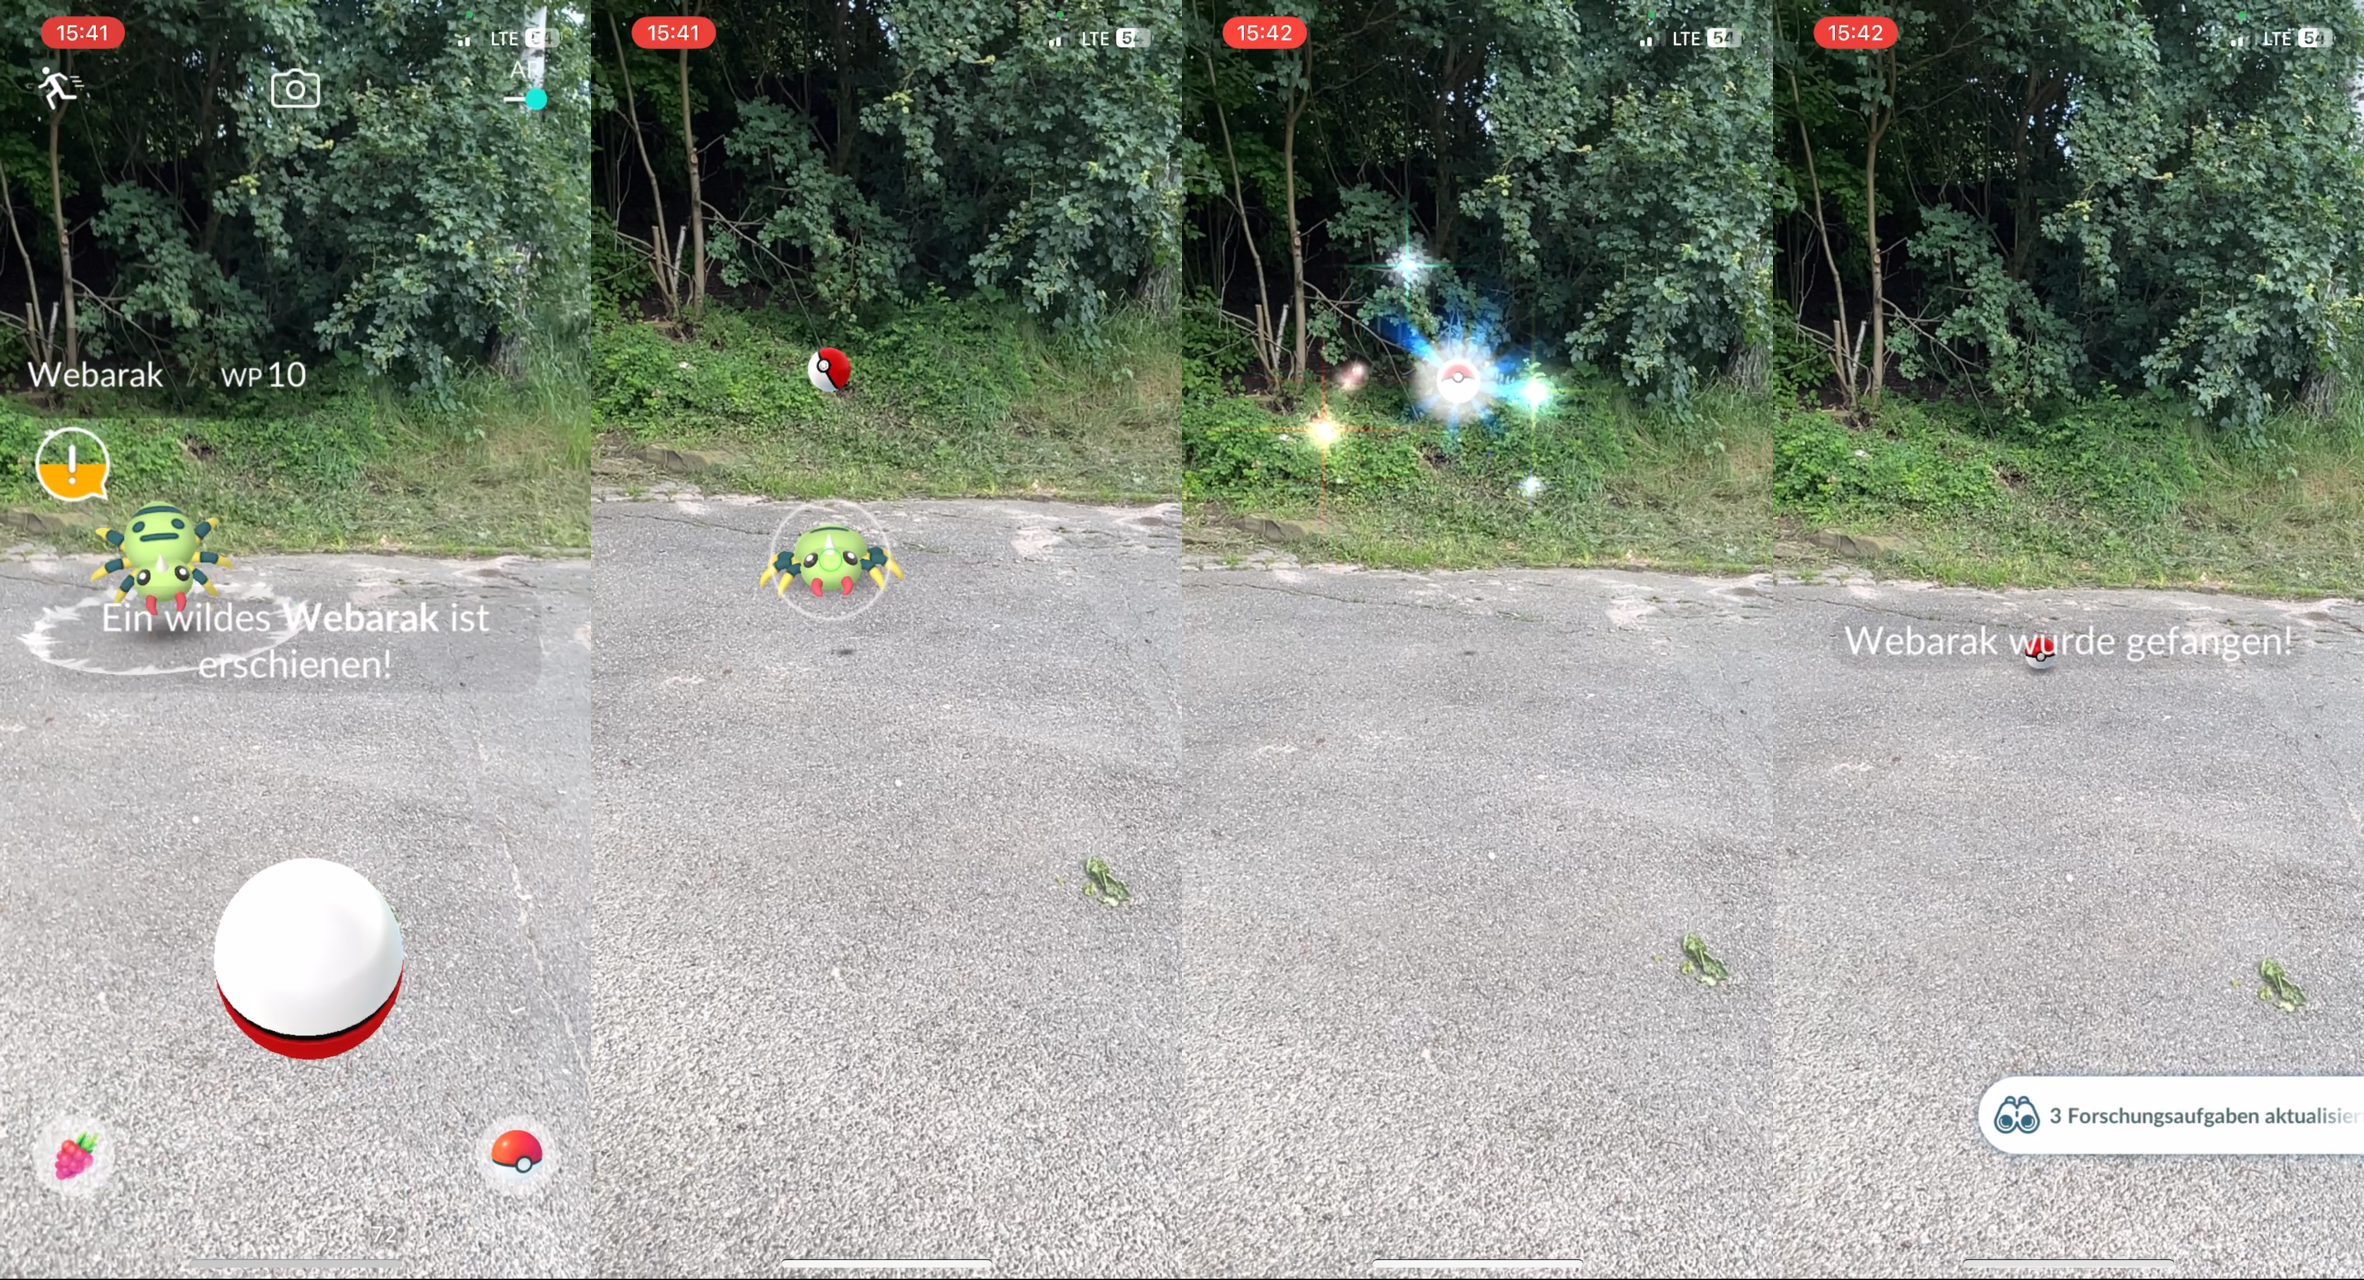
\includegraphics[width=0.9\textwidth]{images/PokemonGo.png}
    \caption{Screenshots aus dem AR-Spiel Pok\'emon Go}
    \label{fig:pokemon-go}
  \end{figure}

  Jedoch ist die Nutzung von Smartphones für AR sehr weit verbreitet, da fast jeder ein Smartphone besitzt und so keine zusätzliche Hardware benötigt wird.
  Beispielsweise hatte das AR-Spiel Pok\'emon Go, welches 2016 veröffentlicht wurde, bereits Anfang 2019 über 1 Milliarde Downloads \autocite[][]{pokemon-go-stats}.
  Bei dem Spiel werden, wie in Darstellung \ref*{fig:pokemon-go} gezeigt ist, sogenannte Pok\'emon über die Smartphone-Kamera in die reale Welt projiziert, sodass der Nutzer sie fangen kann.
  Der Erfolg dieses simplen Konzepts zeigt das Potenzial der riesigen Nutzergruppe von Smartphones für AR-Anwendungen.

  Diese Technologien können auch für praktische Anwendungen genutzt werden, wie bspw. für die Navigation in der Stadt oder für das Ausmessen von Längen mithilfe der Kameras und Sensoren.

  Auch können Smartphones als Displays für HMDs genutzt werden.
  Dabei ist jedoch meist die Kamera des Smartphones nicht mehr nutzbar, wodurch normalerweise nur die Wiedergabe von VR-Inhalten und nicht AR möglich ist.
  Zudem ist die Pixeldichte von Smartphones meist geringer als bei speziellen VR- und AR-Anzeigegeräten, was die Immersion und Nutzererfahrung verschlechtern kann, da das Display sehr nah an den Augen des Nutzers ist und daher starke visuelle Fehler auftreten.

  

  \subsection{Spatial Displays}

  Die bisher vorgestellten Konzepte für AR-Anzeigegeräte basieren auf Displays die direkt am Nutzer selbst befestigt sind.
  Im Kontrast dazu ist die meiste Technik bei Spatial Displays in der Umgebung des Nutzers verbaut.
  Der Nutzer selbst muss dabei keine spezielle Hardware tragen, um die AR-Inhalte zu sehen \autocite[]{bimber2006modern}.
  Jedoch können beispielsweise zur Interaktion mit Inhalten Eingabegeräte genutzt werden, die der Nutzer in der Hand hält.

  Da in vielen Fällen keine spezielle Hardware am Nutzer selbst befestigt werden muss, kann die Immersion durch Spatial Displays sehr hoch sein.
  Auch das ergonomische Nutzererlebnis über lange Zeiträume kann durch Spatial Displays verbessert werden, da der Nutzer nicht durch das Tragen von schwerer Hardware belastet wird.

  Ein Nachteil von Spatial Displays ist der Abstand der Displays zum Nutzer.
  Da sie weiter vom Nutzer entfernt sind als HMDs oder Hand-Held-Devices können sie mit der gleichen Displaygröße nur ein kleineres Sichtfeld abdecken.
  Daher werden bei Spatial Displays oft sehr große Displays bzw. Beamer genutzt, um trotzdem ein großes Sichtfeld abzudecken.
  Dadurch sind Spatial Displays deutlich teurer und aufwendiger in der Installation als HMDs oder Hand-Held-Devices.
  Sie werden daher meist in aufwendigen Anwendungen genutzt und sind für den privaten Gebrauch eher ungeeignet.

  \begin{figure}[H]
    \centering
    \includegraphics[width=0.9\textwidth]{images/merc-sim.png}
    \caption{Innenraum des Mercedes-Benz Fahrsimulators}
    \source{\autocite{MercedesSimulator}}
    \label{fig:merc-sim}
  \end{figure}

  Eine solche Anwendung ist in Abbildung \ref{fig:merc-sim} zu sehen, bei der die kompletten Wände von 14 Projektoren bespielt werden, um eine immersive Umgebung für den Fahrsimulator zu schaffen.
  Die Anzeige der Inhalte ist auf die Fahrerposition des Autos abgestimmt, sodass der Fahrer das Gefühl hat, sich tatsächlich in einem Auto zu befinden.
  Mit solchen hoch entwickelten Spatial Displays können also sehr realistische und immersive Umgebungen geschaffen werden, die für viele Anwendungen, wie bspw. Fahrsimulatoren, sehr nützlich sind aber auch mit extrem hohen Kosten und Aufwand im Vergleich zu anderen Darstellungsmöglichkeiten verbunden sind.

  Betrachtet man Spatial Displays jedoch nicht nur auf Basis der Immersion die durch sie erreicht werden kann, ergeben sich auch viele Anwendungsmöglichkeiten für Spatial Displays, die nicht auf Immersion abzielen.
  Beispielsweise können Spatial Displays genutzt werden, um Informationen in die reale Welt zu projizieren, die für den Nutzer nützlich sind.
  So zählen auch Head-Up-Displays in Autos zu den Spatial Displays, welches Informationen in das Sichtfeld des Fahrers projiziert, ohne dass sich dieser auf ein Display konzentrieren muss.
  Sie nutzen ähnliche Technologien wie Smart-Glasses, um Informationen auf Semi-Transparente Displays zu projizieren.

  
\section{Gamification von UX}
\label{sec:gamification-ux}

\glqq{}Gamification ist die Nutzung von Spielmechanismen und -designprinzipien in nicht-spielerischen Kontexten um das Nutzerengagement zu erhöhen.\grqq{} \autocite[][S.63]{hillmann2021ux} 
So beschreibt Cornel Hillmann, ein Experte für User Experience Design, die Bedeutung von Gamification von UX.

Dieses Prinzip lässt sich aufgrund der hohen Immersion und Interaktivität von VR und AR in XR-Anwendungen besonders gut und quasi standartmäßig nutzen, um das Nutzerengagement zu erhöhen.
Auch durch den Neuheitsfaktor von AR und VR können Nutzer dazu motiviert werden, die Anwendung mehr zu nutzen.

Hillmann gibt er 3 Hauptbestandteile seines Ansatzes von Gamification von UX an, die in einer Anwendung vorhanden sein müssen, um das Nutzerengagement zu erhöhen:
\begin{itemize}
  \item Motivation: Die Anwendung muss Elemente enthalten, die den Nutzer zur weiteren Nutzung motivieren.
  \item Herausforderung: Der Nutzer muss eine Herausforderung haben, die er bewältigen kann.
  \item Trigger: Der Nutzer muss für die Herausforderung belohnt werden.
\end{itemize}
\autocite[S.66]{hillmann2021ux}

Der Ansatz von Hillmann versucht dabei stark, die Belohnungsmechanismen von Spielen zu nutzen, um den Nutzer zu motivieren.
Eine Möglichkeit, die er beschreibt, ist das Nutzen von Punkten, um den Fortschritt des Nutzers zu visualisieren und ihn so zu motivieren, weiterzumachen.

Hillmann beschreibt auch, wie Gamification von UX bei der Orientierung, Beruhigung und Onboarding-Problemen der neuen Technologie von XR helfen kann.
Neue Nutzer schauen beispielsweise oft nicht in die richtige Richtung, um die Inhalte zu sehen, oder sind überfordert von der neuen Technologie.
Daher kann durch intelligente Anrichtung der Objekten und eine spielähnliche Zielführung die Orientierung und User Experience des Nutzers verbessert werden\autocite[S.67]{hillmann2021ux}.